% =============================================================================
% Emergent Behaviour Score (EBS): Technical Document
% Project: Emerge — Life Simulation with Autonomous LLM Agents
% Date: March 2026
% =============================================================================
\documentclass[a4paper, 11pt]{article}

% --- Packages ----------------------------------------------------------------
\usepackage[utf8]{inputenc}
\usepackage[T1]{fontenc}
\usepackage[english]{babel}
\usepackage{amsmath, amssymb, amsthm, mathtools}
\usepackage{booktabs, array, multirow}
\usepackage[margin=2.5cm]{geometry}
\usepackage[colorlinks=true, linkcolor=blue!70!black, citecolor=green!50!black, urlcolor=blue!60!black]{hyperref}
\usepackage{xcolor}
\usepackage{enumitem}
\usepackage[most]{tcolorbox}
\usepackage{graphicx}
\usepackage{rotating}
\usepackage{tikz}
\usepackage{pgfplots}
\pgfplotsset{compat=1.18}
\usetikzlibrary{arrows.meta, positioning, shapes.geometric, calc}

% --- Custom tcolorbox environments ------------------------------------------
\newtcolorbox{keyidea}[1][]{%
    colback=blue!5!white,
    colframe=blue!60!black,
    fonttitle=\bfseries,
    title={Key Idea},
    #1
}

\newtcolorbox{warningbox}[1][]{%
    colback=red!5!white,
    colframe=red!60!black,
    fonttitle=\bfseries,
    title={Warning},
    #1
}

\newtcolorbox{interpretbox}[1][]{%
    colback=green!5!white,
    colframe=green!50!black,
    fonttitle=\bfseries,
    title={Interpretation},
    #1
}

% --- Custom commands ---------------------------------------------------------
\newcommand{\ebs}{\text{EBS}}
\newcommand{\Natt}{N_{\text{att}}}
\newcommand{\Napp}{N_{\text{app}}}
\newcommand{\Nused}{N_{\text{used}}}
\newcommand{\Ncustom}{N_{\text{custom}}}
\newcommand{\Nsuccess}{N_{\text{success}}}
\newcommand{\welfare}{\mathcal{W}}

% --- Title -------------------------------------------------------------------
\title{%
    \textbf{Emergent Behaviour Score (EBS)}:\\[0.5em]
    \Large A Composite Metric for Quantifying Emergent Behaviour\\
    in LLM-Driven Agent Simulations%
}
\author{Emerge Project}
\date{March 2026}

% =============================================================================
\begin{document}
\maketitle
\tableofcontents
\newpage

% =============================================================================
\section{Executive Summary}
% =============================================================================

The Emergent Behaviour Score (EBS) is a composite metric designed to quantify the degree of emergent behaviour in simulation runs of the Emerge project, where autonomous agents controlled by large language models attempt to survive in a procedurally generated 2D world. EBS aggregates six independently computed components---Novelty, Utility, Realization, Stability, Autonomy, and Longevity---into a single score on a 0--100 scale via a weighted sum. Each component captures a distinct dimension of emergence: whether agents invent genuinely new capabilities, whether those inventions improve survival, whether proposals translate into action, whether the agent's internal beliefs remain coherent, whether behaviour is proactive rather than reactive, and whether agents survive long enough to demonstrate sustained emergence. The metric is computed in a single pass over the structured event log (\texttt{events.jsonl}) produced by each simulation run, making it fully deterministic and reproducible.

% =============================================================================
\section{Introduction and Context}
% =============================================================================

The Emerge project is a life simulation in which human-like agents, controlled by large language models (currently Qwen 3.5-35B via vLLM), inhabit a procedurally generated 2D tile-based world. Agents are born with a small set of built-in actions---\texttt{move}, \texttt{eat}, \texttt{rest}, \texttt{innovate}, \texttt{pickup}, \texttt{drop\_item}, \texttt{communicate}, \texttt{give\_item}, and \texttt{teach}---and must manage three survival statistics: life, hunger, and energy.

The simulation's core research question is whether LLM-driven agents can exhibit \emph{emergent behaviour}: capabilities, strategies, and cultural artefacts that are not part of the initial action set and that arise through autonomous reasoning, environmental interaction, and an innovation system. Agents can propose entirely new actions via the \texttt{innovate} command; an Oracle subsystem validates proposals against world rules and precedents, assigning each approved innovation a functional category and a set of requirements and effects. Approved innovations become available as custom actions that any agent can subsequently execute.

Comparing simulation runs across different configurations (model size, prompt strategy, world topology, population size) requires a unified metric that captures the multi-dimensional nature of emergence. A run where agents invent many actions that are never used is qualitatively different from one where a single well-used innovation transforms survival strategy. EBS is designed to capture these distinctions in a single comparable number while preserving the ability to drill into individual components for diagnostic purposes.

\paragraph{What EBS does not capture.}
EBS measures \emph{intra-run} emergence quality. It does not measure inter-agent social dynamics (beyond what is reflected in innovation categories), knowledge transfer fidelity, or aesthetic qualities of agent behaviour. It is not a measure of simulation ``goodness''---a research question about reactive survival is best served by a run with low EBS.

% =============================================================================
\section{Problem Motivating the Metric}
% =============================================================================

Simple scalar metrics fail to capture the multi-dimensional nature of emergence:

\begin{itemize}[nosep]
    \item \textbf{Raw innovation count} rewards quantity over quality. An agent that proposes 50 trivial renaming actions scores higher than one that invents a single transformative tool.
    \item \textbf{Survival time} conflates good environment design with agent capability. Agents on a resource-rich map survive long without innovating.
    \item \textbf{Action diversity} (e.g., Shannon entropy of the action distribution) does not distinguish meaningful innovation from noise---parse failures and hallucinated actions inflate diversity.
    \item \textbf{Simple success rate} ignores whether successful actions are novel or merely the same \texttt{eat}/\texttt{rest} loop.
\end{itemize}

Emergence is inherently multi-dimensional: novelty alone does not constitute useful emergence; utility without novelty is just effective use of built-in actions; novelty with utility but without realization means ideas that never materialise. A composite metric is therefore necessary.

% =============================================================================
\section{Intuition Behind the Metric}
% =============================================================================

EBS functions as a ``report card'' across six dimensions of emergent behaviour. Each component independently assesses one aspect, and the final score is a weighted sum reflecting research priorities.

\begin{keyidea}
    Emergence $=$ \textbf{Novelty} (are agents inventing new things?) $+$ \textbf{Utility} (do inventions help?) $+$ \textbf{Realization} (do ideas become actions?) $+$ \textbf{Stability} (is the agent's world model coherent?) $+$ \textbf{Autonomy} (is behaviour proactive and goal-directed?) $+$ \textbf{Longevity} (do agents survive long enough to demonstrate emergence?)
\end{keyidea}

The weighted-sum design means that components are \emph{independent assessments}: a run can score high on Novelty but low on Realization (many ideas, few executed), or high on Stability but low on Novelty (coherent agent that never innovates). The weights express the relative importance assigned to each dimension by the research team and are design choices, not empirically derived constants.

% =============================================================================
\section{Definitions and Notation}
% =============================================================================

Table~\ref{tab:notation} lists all symbols used in the EBS formulation.

\begin{table}[ht]
\centering
\caption{Symbol definitions.}
\label{tab:notation}
\begin{tabular}{@{}lp{10cm}@{}}
\toprule
\textbf{Symbol} & \textbf{Definition} \\
\midrule
$\Natt$ & Number of innovation attempts in the run \\
$\Napp$ & Number of approved (validated) innovations \\
$\Nused$ & Number of approved innovations that were subsequently executed at least once \\
$\Ncustom$ & Total number of custom action executions across all agents \\
$\Nsuccess$ & Number of successful custom action executions \\
$w_k$ & Weight of component $k$ in the EBS formula ($\sum w_k = 1$) \\
$C_k$ & Score of component $k$, normalised to $[0, 100]$ \\
$\welfare(t)$ & Welfare function at tick $t$: $\text{life}(t) + \text{energy}(t) - \text{hunger}(t)$ \\
$\lambda$ & Longevity reference constant (agent-ticks); default $= 1500$ \\
$T_{\text{agent}}$ & Total agent-ticks: $\sum_{\text{agents}} (\text{ticks alive})$ \\
$T$ & Total ticks in the run \\
$A_0$ & Number of agents at run start (initial population) \\
\bottomrule
\end{tabular}
\end{table}

\paragraph{Key terms.}
An \textbf{innovation} is a new action proposed by an agent via the \texttt{innovate} command and validated by the Oracle. A \textbf{custom action} is any execution of an approved innovation. The \textbf{welfare function} $\welfare$ is defined as $\text{life} + \text{energy} - \text{hunger}$, capturing overall agent well-being as a single scalar. The \textbf{approval rate} is the fraction of innovation attempts that the Oracle approves.

% =============================================================================
\section{Formal Definition}
% =============================================================================

The Emergent Behaviour Score is defined as:

\begin{equation}
\boxed{\;
\ebs = \sum_{k=1}^{6} w_k \cdot C_k
\;}
\label{eq:ebs}
\end{equation}

\noindent where the six components and their weights are:

\begin{table}[ht]
\centering
\caption{EBS component weights.}
\label{tab:weights}
\begin{tabular}{@{}llc@{}}
\toprule
$k$ & \textbf{Component} & $w_k$ \\
\midrule
1 & Novelty     & 0.25 \\
2 & Utility     & 0.17 \\
3 & Realization & 0.17 \\
4 & Stability   & 0.13 \\
5 & Autonomy    & 0.13 \\
6 & Longevity   & 0.15 \\
\midrule
  & \textbf{Total} & \textbf{1.00} \\
\bottomrule
\end{tabular}
\end{table}

Each component $C_k \in [0, 100]$. Consequently, $\ebs \in [0, 100]$.

% --- 6.1 Novelty -------------------------------------------------------------
\subsection{Novelty ($w = 0.25$)}

Novelty measures the degree to which agents invent genuinely new actions beyond the built-in set.

\begin{equation}
C_{\text{novelty}} = 100 \left(
    0.40 \cdot \underbrace{\frac{\Napp}{\Natt}}_{\text{approval rate}}
    + 0.30 \cdot \underbrace{\frac{|\mathcal{K}|}{4}}_{\text{category diversity}}
    + 0.30 \cdot \underbrace{\frac{N_{\text{non-base}}}{\Napp}}_{\text{structural originality}}
\right)
\label{eq:novelty}
\end{equation}

\paragraph{Approval rate} $= \Napp / \Natt$. The fraction of innovation proposals that the Oracle accepts. Rewards agents that propose well-formed, plausible actions.

\paragraph{Category diversity.} $\mathcal{K}$ is the set of distinct functional categories among approved innovations. The Oracle assigns each approved innovation to one of four categories:

\begin{enumerate}[nosep]
    \item \textsc{survival} --- actions directly improving survival stats
    \item \textsc{crafting} --- actions that create or transform items
    \item \textsc{exploration} --- actions related to movement or perception
    \item \textsc{social} --- actions involving other agents
\end{enumerate}

Category diversity is $|\mathcal{K}| / 4$, rewarding breadth of innovation across functional domains.

\paragraph{Structural originality.} $N_{\text{non-base}}$ counts approved innovations whose structural novelty tag is \emph{not} \texttt{base\_extension} (see Appendix~\ref{app:structural} for classification rules). This rewards innovations that introduce genuinely new capabilities (item production, recipes, world modification, coordination) rather than simple extensions of existing stat-modifying actions.

\paragraph{Edge cases.} If $\Natt = 0$, approval rate defaults to $0$. If $\Napp = 0$, both category diversity and structural originality default to $0$.

% --- 6.2 Utility --------------------------------------------------------------
\subsection{Utility ($w = 0.17$)}

Utility measures whether innovations produce measurable advantages for agent survival.

\begin{equation}
C_{\text{utility}} = 100 \left(
    0.50 \cdot \underbrace{\frac{N_{\Delta^+}}{\Nused}}_{\text{direct state improvement}}
    + 0.30 \cdot \underbrace{\frac{N_{\text{items}}}{\Napp}}_{\text{future option value}}
    + 0.20 \cdot \underbrace{\frac{\Nsuccess}{\Ncustom}}_{\text{execution success rate}}
\right)
\label{eq:utility}
\end{equation}

\paragraph{Direct state improvement.} For each used innovation, the welfare delta $\Delta\welfare$ is computed by comparing the mean welfare across all agents in a 5-tick window before and after the innovation's first execution:
\begin{align}
    \bar{\welfare}_{\text{before}} &= \frac{1}{|S_{\text{before}}|} \sum_{s \in S_{\text{before}}} \welfare(s) \label{eq:welfare_before} \\
    \bar{\welfare}_{\text{after}}  &= \frac{1}{|S_{\text{after}}|}  \sum_{s \in S_{\text{after}}}  \welfare(s) \label{eq:welfare_after} \\
    \Delta\welfare &= \bar{\welfare}_{\text{after}} - \bar{\welfare}_{\text{before}}
\end{align}

\noindent where $S_{\text{before}} = \{s : t_{\text{first}} - 5 \leq s.\text{tick} < t_{\text{first}}\}$ and $S_{\text{after}} = \{s : t_{\text{first}} \leq s.\text{tick} < t_{\text{first}} + 5\}$, aggregated across \emph{all} agents' state histories. $N_{\Delta^+}$ counts innovations where $\Delta\welfare > 0$.

\paragraph{Future option value.} $N_{\text{items}}$ counts approved innovations whose \texttt{produces} field contains at least one non-stat key (i.e., keys other than \texttt{hunger}, \texttt{energy}, \texttt{life}, \texttt{health}). This captures innovations that create inventory items, enabling future crafting or tool use.

\paragraph{Execution success rate.} $\Nsuccess / \Ncustom$ across all custom action executions in the run.

\paragraph{Edge cases.} If $\Nused = 0$, direct state improvement defaults to $0$. If $\Napp = 0$, future option value defaults to $0$. If $\Ncustom = 0$, execution success rate defaults to $0$.

% --- 6.3 Realization ----------------------------------------------------------
\subsection{Realization ($w = 0.17$)}

Realization measures whether innovations move from proposal to execution---the gap between ideas and action.

\begin{equation}
C_{\text{realization}} = 100 \left(
    0.60 \cdot \underbrace{\frac{\Nused}{\Napp}}_{\text{use rate}}
    + 0.40 \cdot \underbrace{\frac{\Nsuccess}{\Ncustom}}_{\text{execution success rate}}
\right)
\label{eq:realization}
\end{equation}

\paragraph{Use rate.} Fraction of approved innovations that are executed at least once by any agent. A high approval count with low use rate indicates a ``proposal--execution gap'': agents invent actions they never employ.

\paragraph{Execution success rate.} Shared with Utility; measures whether custom actions succeed when attempted.

\paragraph{Edge cases.} If $\Napp = 0$, use rate defaults to $0$. If $\Ncustom = 0$, execution success rate defaults to $0$.

% --- 6.4 Stability ------------------------------------------------------------
\subsection{Stability ($w = 0.13$)}

Stability measures the internal coherence of agents' belief systems. Unlike the other components, Stability uses a \emph{penalty} model: it starts at 100 and is reduced by coherence failures.

\begin{equation}
C_{\text{stability}} = \text{clamp}\!\left(
    100
    - 40 \cdot \underbrace{\frac{N_{\text{contradictions}}}{N_{\text{learnings}}}}_{\text{false knowledge rate}}
    - 30 \cdot \underbrace{\frac{N_{\text{parse fails}}}{N_{\text{actions}}}}_{\text{invalid action rate}}
    ,\; 0,\; 100
\right)
\label{eq:stability}
\end{equation}

\paragraph{False knowledge rate.} $N_{\text{contradictions}}$ counts learnings (from memory compression events) that contradict ground-truth facts established during the run. Contradiction detection uses pattern matching:
\begin{itemize}[nosep]
    \item \textbf{Resource denial}: a learning claims ``no $X$'' / ``$X$ not found'' / ``can't find $X$'' for a resource $X$ that was confirmed consumed or picked up.
    \item \textbf{Action denial}: a learning claims ``$X$ never works'' / ``$X$ doesn't work'' for an action $X$ that succeeded at least once.
\end{itemize}

\paragraph{Invalid action rate.} $N_{\text{parse fails}}$ counts agent decisions where the LLM output could not be parsed into a valid action (malformed JSON, unknown action names, etc.).

\paragraph{Note on contradiction rate.} In the current implementation, \texttt{contradiction\_rate} is unified with \texttt{false\_knowledge\_rate} (i.e., they are the same value). The maximum possible penalty is therefore $40 + 30 = 70$ points, leaving a theoretical minimum Stability of $30$ even under worst-case conditions.

% --- 6.5 Autonomy -------------------------------------------------------------
\subsection{Autonomy ($w = 0.13$)}

Autonomy measures proactive, goal-directed behaviour as opposed to purely reactive survival.

\begin{equation}
C_{\text{autonomy}} = 100 \left(
    0.40 \cdot \underbrace{r_{\text{proactive}}}_{\substack{\text{proactive resource} \\ \text{acquisition}}}
    + 0.30 \cdot \underbrace{r_{\text{contingent}}}_{\substack{\text{environment-contingent} \\ \text{innovation}}}
    + 0.30 \cdot \underbrace{r_{\text{subgoals}}}_{\substack{\text{self-generated} \\ \text{subgoals}}}
\right)
\label{eq:autonomy}
\end{equation}

\begin{warningbox}
    In the current implementation, $r_{\text{subgoals}} = 0$ always (placeholder for future semantic analysis of agent reasoning). The effective maximum Autonomy score is therefore $\mathbf{70}$, not $100$.
\end{warningbox}

\paragraph{Proactive resource acquisition ($r_{\text{proactive}}$).} Fraction of move actions that are ``proactive'': the agent moves \emph{toward} a nearby resource while its hunger is \emph{below} the threshold of $60$ (i.e., not urgently hungry). Specifically, a move is proactive if:
\begin{enumerate}[nosep]
    \item The action is \texttt{move} with a recognised direction.
    \item The agent's hunger at that tick is $< 60$.
    \item There exists a resource in the agent's perception whose relative position $(\Delta x, \Delta y)$ matches the movement direction.
\end{enumerate}

\paragraph{Environment-contingent innovation ($r_{\text{contingent}}$).} Fraction of innovation attempts that occur when the agent's hunger is $> 60$. This captures innovation driven by environmental pressure rather than idle experimentation.

\paragraph{Self-generated subgoals ($r_{\text{subgoals}}$).} Intended to capture multi-step planning inferred from agent reasoning. Currently always $0$; will require semantic analysis of agent decision traces in a future version.

% --- 6.6 Longevity ------------------------------------------------------------
\subsection{Longevity ($w = 0.15$)}

Longevity measures whether agents survive long enough to demonstrate sustained emergent behaviour.

\begin{equation}
C_{\text{longevity}} = 100 \left(
    0.50 \cdot \underbrace{\frac{T_{\text{agent}}}{A_0 \cdot T}}_{\text{population vitality}}
    + 0.50 \cdot \underbrace{\left(1 - e^{-T_{\text{agent}} / \lambda}\right)}_{\text{absolute longevity}}
\right)
\label{eq:longevity}
\end{equation}

\paragraph{Population vitality.} The ratio of actual agent-ticks lived to the maximum possible (if all initial agents survived the entire run). A value of $1.0$ means no agent died; $0.5$ means half the potential lifespan was realised.

\paragraph{Absolute longevity.} An exponential asymptotic function of total agent-ticks. The reference constant $\lambda = 1500$ represents a baseline expectation of approximately 3 agents $\times$ 500 ticks. The function $f(x) = 1 - e^{-x/\lambda}$ has these properties:
\begin{itemize}[nosep]
    \item $f(0) = 0$: no survival $\Rightarrow$ zero score.
    \item $f(\lambda) = 1 - e^{-1} \approx 0.632$: reaching the baseline yields $\approx 63\%$ of the maximum.
    \item $f \to 1$ as $x \to \infty$: diminishing returns on very long runs, preventing Longevity from dominating.
\end{itemize}

\paragraph{Edge cases.} If $A_0 = 0$ or $T = 0$, population vitality defaults to $0$.

% =============================================================================
\section{Computation Procedure}
\label{sec:computation}
% =============================================================================

EBS is computed in a \textbf{single pass} over the event stream (\texttt{events.jsonl}), followed by a scoring phase. The algorithm proceeds as follows:

\begin{enumerate}
    \item \textbf{Initialise accumulators}: innovation registry, custom action log, per-agent state/perception/decision histories, learnings log, ground-truth sets for contradiction detection, and scalar counters (parse failures, action totals, attempt/approval counts, agent-tick totals).

    \item \textbf{Stream events}: read \texttt{events.jsonl} line by line. For each event, update the relevant accumulators based on \texttt{event\_type}:
    \begin{itemize}[nosep]
        \item \texttt{run\_start}: extract initial agent count and run ID.
        \item \texttt{agent\_decision}: increment action count; flag parse failures.
        \item \texttt{agent\_state}: record survival state per agent per tick.
        \item \texttt{agent\_perception}: record hunger and nearby resources.
        \item \texttt{oracle\_resolution}: update ground-truth resource/action sets.
        \item \texttt{innovation\_attempt}: increment attempt counter; tag hunger state.
        \item \texttt{innovation\_validated}: register approved innovations.
        \item \texttt{custom\_action\_executed}: mark innovations as used; log success/failure.
        \item \texttt{memory\_compression\_result}: collect learnings for contradiction detection.
        \item \texttt{run\_end}: record total ticks.
    \end{itemize}

    \item \textbf{Post-pass classification}: for each approved innovation, classify structural novelty (Appendix~\ref{app:structural}) and dependency depth. Compute welfare deltas for used innovations.

    \item \textbf{Contradiction detection}: for each learning, check against ground-truth sets using pattern matching.

    \item \textbf{Score computation}: compute each of the six component scores using the formulas in Section~6, then combine via the weighted sum.

    \item \textbf{Output}: write \texttt{metrics/ebs.json} containing the overall EBS score, per-component scores and sub-scores, and the innovation registry.
\end{enumerate}

\paragraph{Input.} \texttt{data/runs/<run\_id>/events.jsonl} --- one JSON object per line.

\paragraph{Output.} \texttt{data/runs/<run\_id>/metrics/ebs.json} --- structured JSON with scores at all levels.

\vspace{1em}
Figure~\ref{fig:dataflow} illustrates the data flow from events to the final EBS score.

\begin{sidewaysfigure}
\centering
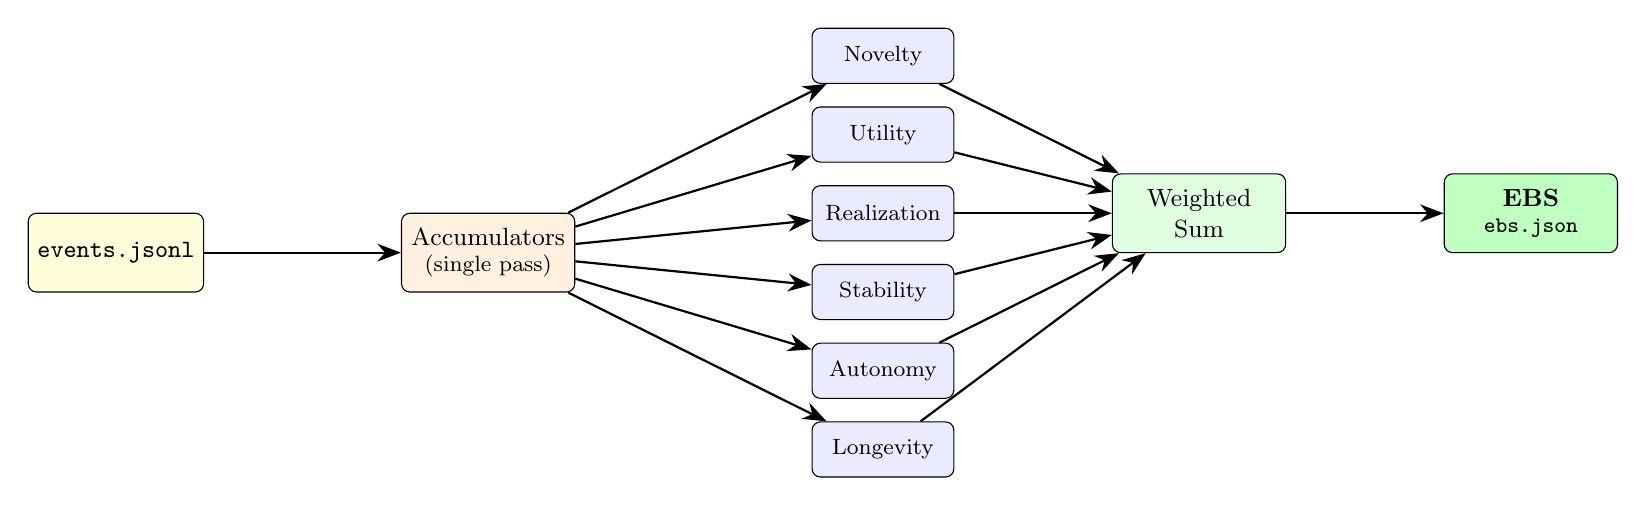
\begin{tikzpicture}[
    node distance=1.8cm and 2.5cm,
    box/.style={rectangle, draw, rounded corners=3pt, minimum height=1cm,
                minimum width=2.2cm, align=center, font=\small},
    compbox/.style={rectangle, draw, rounded corners=3pt, minimum height=0.7cm,
                    minimum width=1.8cm, align=center, font=\footnotesize,
                    fill=blue!8},
    arr/.style={-{Stealth[length=3mm]}, thick},
]
    % Input
    \node[box, fill=yellow!15] (events) {\texttt{events.jsonl}};

    % Accumulators
    \node[box, fill=orange!12, right=2.5cm of events] (accum) {Accumulators\\[-0.2em]\footnotesize (single pass)};

    % Component scores
    \node[compbox, right=3cm of accum, yshift=2.5cm]  (nov) {Novelty};
    \node[compbox, right=3cm of accum, yshift=1.5cm]  (utl) {Utility};
    \node[compbox, right=3cm of accum, yshift=0.5cm]  (rea) {Realization};
    \node[compbox, right=3cm of accum, yshift=-0.5cm] (sta) {Stability};
    \node[compbox, right=3cm of accum, yshift=-1.5cm] (aut) {Autonomy};
    \node[compbox, right=3cm of accum, yshift=-2.5cm] (lon) {Longevity};

    % Weighted sum
    \node[box, fill=green!12, right=2cm of rea] (wsum) {Weighted\\Sum};

    % Output
    \node[box, fill=green!25, right=2cm of wsum] (ebs) {\textbf{EBS}\\[-0.2em]\footnotesize \texttt{ebs.json}};

    % Arrows: events -> accum
    \draw[arr] (events) -- (accum);

    % Arrows: accum -> components
    \foreach \comp in {nov, utl, rea, sta, aut, lon} {
        \draw[arr] (accum) -- (\comp);
    }

    % Arrows: components -> weighted sum
    \foreach \comp in {nov, utl, rea, sta, aut, lon} {
        \draw[arr] (\comp) -- (wsum);
    }

    % Arrow: weighted sum -> EBS
    \draw[arr] (wsum) -- (ebs);
\end{tikzpicture}
\caption{Data flow: events are streamed into accumulators in a single pass, six component scores are computed, and the weighted sum produces the final EBS.}
\label{fig:dataflow}
\end{sidewaysfigure}

% =============================================================================
\section{Score Interpretation}
\label{sec:interpretation}
% =============================================================================

% --- 8.1 How to read --------------------------------------------------------
\subsection{How to Read This Metric in Practice}

The single EBS number provides a quick comparison between runs, but the real diagnostic value lies in the \textbf{component breakdown}. When comparing two runs:

\begin{enumerate}[nosep]
    \item Compare overall EBS for a high-level ranking.
    \item Examine the six component scores to understand \emph{why} one run scored higher.
    \item Drill into sub-scores (e.g., approval rate vs.\ structural originality within Novelty) to identify specific strengths and weaknesses.
\end{enumerate}

A radar chart (see Section~\ref{sec:examples}, Figure~\ref{fig:radar}) provides an effective visual comparison of component profiles across runs.

% --- 8.2 Interpretation table ------------------------------------------------
\subsection{Interpretation Table}

\begin{interpretbox}
    The thresholds below are \textbf{working assumptions pending empirical calibration}. They are based on design expectations and early testing, not on a statistically validated corpus of runs. Treat them as rough guides, not hard boundaries.
\end{interpretbox}

\begin{table}[ht]
\centering
\caption{EBS interpretation tiers (working assumptions).}
\label{tab:interpretation}
\begin{tabular}{@{}cl p{8cm}@{}}
\toprule
\textbf{EBS Range} & \textbf{Behaviour Tier} & \textbf{Description} \\
\midrule
0--25   & Reactive survival & Agents use only built-in actions. No meaningful innovation or proactive behaviour. \\
26--50  & Proto-emergence & Some innovation attempts; a few may succeed. Behaviour is mostly reactive with sporadic novelty. \\
51--70  & Functional emergence & Multiple useful innovations are proposed, approved, and executed. Agents show signs of proactive behaviour. \\
71--85  & Technological ecology & Diverse innovations across categories, with technology chains and positive survival impact. Proactive, coherent agents. \\
86--100 & Open-ended cultural evolution & Rich innovation ecosystem with deep dependency chains, high realization, and sustained autonomous behaviour. \\
\bottomrule
\end{tabular}
\end{table}

% --- 8.3 Common mistakes -----------------------------------------------------
\subsection{Common Interpretation Mistakes}

\begin{warningbox}[title={Common Pitfalls}]
\begin{enumerate}[nosep]
    \item \textbf{High EBS $\neq$ ``good'' simulation.} EBS measures emergence intensity, not whether the run answers your research question. A study of reactive survival \emph{expects} low EBS.
    \item \textbf{Low Stability with high Novelty $=$ hallucinating agent, not creative agent.} If an agent invents many actions but holds contradictory beliefs, the ``novelty'' may be driven by incoherent reasoning rather than genuine creativity.
    \item \textbf{Autonomy's $r_{\text{subgoals}}$ is always $0$.} The current maximum Autonomy score is $70/100$. Do not interpret Autonomy $= 70$ as ``imperfect autonomy''---it is the theoretical ceiling in the current version.
    \item \textbf{Longevity can mask poor emergence.} If agents survive the entire run but never innovate, Longevity will contribute significantly to EBS while all other components are near zero. Always check the component breakdown.
\end{enumerate}
\end{warningbox}

% =============================================================================
\section{Step-by-Step Numerical Examples}
\label{sec:examples}
% =============================================================================

We present two pedagogically constructed examples with round numbers. These do not represent real simulation data.

% --- Example 1 ---------------------------------------------------------------
\subsection{Example 1: Low-Emergence Run}

\paragraph{Scenario.} 3 agents, 100 ticks. Agents mostly eat and rest. Two innovation attempts, neither approved. Frequent parse failures. No proactive behaviour.

\begin{table}[ht]
\centering
\small
\caption{Example 1: raw data.}
\begin{tabular}{@{}ll@{}}
\toprule
\textbf{Parameter} & \textbf{Value} \\
\midrule
Agents / Ticks & 3 / 100 \\
Innovation attempts / approved & 2 / 0 \\
Total actions / parse failures & 50 / 10 \\
Total learnings / contradictions & 5 / 1 \\
Total moves / proactive moves & 25 / 0 \\
Env-contingent innovation attempts & 0 of 2 \\
Agent-ticks alive (A, B, C) & 100 + 80 + 60 = 240 \\
\bottomrule
\end{tabular}
\end{table}

\paragraph{Novelty.} $\Natt = 2$, $\Napp = 0$. All sub-scores are $0$.
\[
    C_{\text{novelty}} = 100(0.40 \cdot 0 + 0.30 \cdot 0 + 0.30 \cdot 0) = \mathbf{0.00}
\]

\paragraph{Utility.} No approved innovations, no custom actions. All sub-scores are $0$.
\[
    C_{\text{utility}} = \mathbf{0.00}
\]

\paragraph{Realization.} No approved innovations, no custom actions. All sub-scores are $0$.
\[
    C_{\text{realization}} = \mathbf{0.00}
\]

\paragraph{Stability.}
\begin{align*}
    \text{false\_knowledge\_rate} &= 1/5 = 0.20 \\
    \text{invalid\_action\_rate} &= 10/50 = 0.20 \\
    C_{\text{stability}} &= \text{clamp}(100 - 40 \times 0.20 - 30 \times 0.20) = 100 - 8 - 6 = \mathbf{86.00}
\end{align*}

\paragraph{Autonomy.} No proactive moves, no environment-contingent innovation.
\[
    C_{\text{autonomy}} = 100(0.40 \cdot 0 + 0.30 \cdot 0) = \mathbf{0.00}
\]

\paragraph{Longevity.}
\begin{align*}
    T_{\text{agent}} &= 240, \quad A_0 = 3, \quad T = 100 \\
    \text{population\_vitality} &= 240 / (3 \times 100) = 0.80 \\
    \text{absolute\_longevity} &= 1 - e^{-240/1500} = 1 - e^{-0.16} \approx 0.148 \\
    C_{\text{longevity}} &= 100(0.50 \times 0.80 + 0.50 \times 0.148) = 100(0.400 + 0.074) = \mathbf{47.40}
\end{align*}

\paragraph{Final EBS.}
\begin{align*}
    \ebs &= 0.25 \times 0 + 0.17 \times 0 + 0.17 \times 0 + 0.13 \times 86.00 + 0.13 \times 0 + 0.15 \times 47.40 \\
    &= 0 + 0 + 0 + 11.18 + 0 + 7.11 = \boxed{18.29}
\end{align*}

\begin{interpretbox}
    EBS $\approx 18$ falls in the \textbf{reactive survival} tier. The only positive contributions come from Stability (agents are somewhat coherent despite some contradictions and parse failures) and Longevity (agents survived a reasonable fraction of the run). Zero innovation success means zero Novelty, Utility, and Realization.
\end{interpretbox}

% --- Example 2 ---------------------------------------------------------------
\subsection{Example 2: Rich-Emergence Run}

\paragraph{Scenario.} 3 agents, 200 ticks. Diverse innovations across all four categories, most of which are used successfully. Proactive resource-seeking behaviour. All agents survive the full run.

\begin{table}[ht]
\centering
\small
\caption{Example 2: raw data.}
\begin{tabular}{@{}ll@{}}
\toprule
\textbf{Parameter} & \textbf{Value} \\
\midrule
Agents / Ticks & 3 / 200 \\
Innovation attempts / approved & 10 / 8 \\
Categories represented & 4 of 4 \\
Non-\texttt{base\_extension} innovations & 5 of 8 \\
Used innovations & 6 of 8 \\
Custom action executions / successes & 20 / 16 \\
Innovations with $\Delta\welfare > 0$ & 4 of 6 used \\
Innovations producing items & 3 of 8 \\
Total actions / parse failures & 100 / 5 \\
Total learnings / contradictions & 10 / 0 \\
Total moves / proactive moves & 80 / 50 \\
Env-contingent innovation attempts & 6 of 10 \\
Agent-ticks alive (A, B, C) & 200 + 200 + 200 = 600 \\
\bottomrule
\end{tabular}
\end{table}

\paragraph{Novelty.}
\begin{align*}
    \text{approval\_rate} &= 8/10 = 0.80 \\
    \text{category\_diversity} &= 4/4 = 1.00 \\
    \text{structural\_originality} &= 5/8 = 0.625 \\
    C_{\text{novelty}} &= 100(0.40 \times 0.80 + 0.30 \times 1.00 + 0.30 \times 0.625) \\
    &= 100(0.320 + 0.300 + 0.1875) = \mathbf{80.75}
\end{align*}

\paragraph{Utility.}
\begin{align*}
    \text{direct\_state\_improvement} &= 4/6 \approx 0.667 \\
    \text{future\_option\_value} &= 3/8 = 0.375 \\
    \text{execution\_success\_rate} &= 16/20 = 0.80 \\
    C_{\text{utility}} &= 100(0.50 \times 0.667 + 0.30 \times 0.375 + 0.20 \times 0.80) \\
    &= 100(0.333 + 0.113 + 0.160) = \mathbf{60.58}
\end{align*}

\paragraph{Realization.}
\begin{align*}
    \text{use\_rate} &= 6/8 = 0.75 \\
    \text{execution\_success\_rate} &= 16/20 = 0.80 \\
    C_{\text{realization}} &= 100(0.60 \times 0.75 + 0.40 \times 0.80) = 100(0.450 + 0.320) = \mathbf{77.00}
\end{align*}

\paragraph{Stability.}
\begin{align*}
    \text{false\_knowledge\_rate} &= 0/10 = 0 \\
    \text{invalid\_action\_rate} &= 5/100 = 0.05 \\
    C_{\text{stability}} &= 100 - 40 \times 0 - 30 \times 0.05 = 100 - 1.50 = \mathbf{98.50}
\end{align*}

\paragraph{Autonomy.}
\begin{align*}
    r_{\text{proactive}} &= 50/80 = 0.625 \\
    r_{\text{contingent}} &= 6/10 = 0.60 \\
    C_{\text{autonomy}} &= 100(0.40 \times 0.625 + 0.30 \times 0.60) = 100(0.250 + 0.180) = \mathbf{43.00}
\end{align*}

\paragraph{Longevity.}
\begin{align*}
    T_{\text{agent}} &= 600, \quad A_0 = 3, \quad T = 200 \\
    \text{population\_vitality} &= 600 / (3 \times 200) = 1.00 \\
    \text{absolute\_longevity} &= 1 - e^{-600/1500} = 1 - e^{-0.40} \approx 0.330 \\
    C_{\text{longevity}} &= 100(0.50 \times 1.00 + 0.50 \times 0.330) = 100(0.500 + 0.165) = \mathbf{66.50}
\end{align*}

\paragraph{Final EBS.}
\begin{align*}
    \ebs &= 0.25 \times 80.75 + 0.17 \times 60.58 + 0.17 \times 77.00 \\
    &\quad + 0.13 \times 98.50 + 0.13 \times 43.00 + 0.15 \times 66.50 \\
    &= 20.19 + 10.30 + 13.09 + 12.81 + 5.59 + 9.98 = \boxed{71.96}
\end{align*}

\begin{interpretbox}
    EBS $\approx 72$ falls in the \textbf{technological ecology} tier. Strong Novelty and near-perfect Stability drive the score. Autonomy is moderate at $43/70$ (effective ceiling), reflecting good proactive behaviour. Longevity benefits from full population survival but is tempered by the asymptotic function ($\text{absolute\_longevity} \approx 0.33$ at 600 agent-ticks vs.\ the $\lambda = 1500$ baseline).
\end{interpretbox}

% --- Side-by-side comparison --------------------------------------------------
\subsection{Comparison Summary}

\begin{table}[ht]
\centering
\caption{Side-by-side comparison of the two examples.}
\label{tab:comparison}
\begin{tabular}{@{}l rr rr@{}}
\toprule
& \multicolumn{2}{c}{\textbf{Example 1}} & \multicolumn{2}{c}{\textbf{Example 2}} \\
\cmidrule(lr){2-3} \cmidrule(lr){4-5}
\textbf{Component} & Score & Weighted & Score & Weighted \\
\midrule
Novelty ($\times 0.25$)     &  0.00 &  0.00 & 80.75 & 20.19 \\
Utility ($\times 0.17$)     &  0.00 &  0.00 & 60.58 & 10.30 \\
Realization ($\times 0.17$) &  0.00 &  0.00 & 77.00 & 13.09 \\
Stability ($\times 0.13$)   & 86.00 & 11.18 & 98.50 & 12.81 \\
Autonomy ($\times 0.13$)    &  0.00 &  0.00 & 43.00 &  5.59 \\
Longevity ($\times 0.15$)   & 47.40 &  7.11 & 66.50 &  9.98 \\
\midrule
\textbf{EBS}                &       & \textbf{18.29} &  & \textbf{71.96} \\
\bottomrule
\end{tabular}
\end{table}

% --- Radar chart --------------------------------------------------------------
Figure~\ref{fig:radar} shows the component profiles of both examples as a radar chart.

\begin{figure}[ht]
\centering
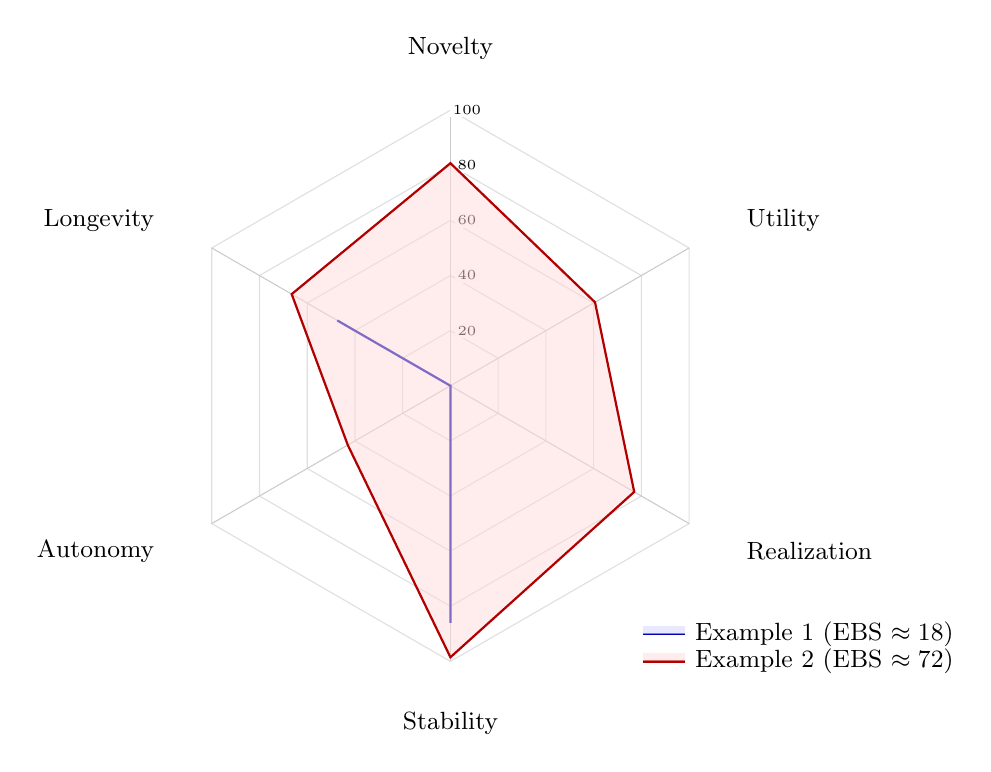
\begin{tikzpicture}[scale=0.035]
    % Configuration
    \def\numaxes{6}
    \def\maxval{100}

    % Axis angles (starting from top, clockwise)
    % Novelty=90, Utility=30, Realization=-30, Stability=-90, Autonomy=-150, Longevity=150
    \def\angles{{90, 30, -30, -90, -150, 150}}

    % Labels
    \def\labels{{"Novelty", "Utility", "Realization", "Stability", "Autonomy", "Longevity"}}

    % Grid levels
    \foreach \level in {20, 40, 60, 80, 100} {
        \draw[gray!25, thin]
            ({cos(\angles[0])*\level}, {sin(\angles[0])*\level})
            \foreach \i in {1,...,5} {
                -- ({cos(\angles[\i])*\level}, {sin(\angles[\i])*\level})
            } -- cycle;
    }

    % Axis lines
    \foreach \i in {0,...,5} {
        \draw[gray!40, thin] (0,0) -- ({cos(\angles[\i])*\maxval}, {sin(\angles[\i])*\maxval});
    }

    % Grid level labels (on the Novelty axis)
    \foreach \level in {20, 40, 60, 80, 100} {
        \node[font=\tiny, fill=white, inner sep=1pt] at ({cos(90)*\level + 6}, {sin(90)*\level}) {\level};
    }

    % Axis labels
    \node[font=\small, above]           at ({cos(90)*115},  {sin(90)*115})  {Novelty};
    \node[font=\small, right]           at ({cos(30)*120},  {sin(30)*120})  {Utility};
    \node[font=\small, right]           at ({cos(-30)*120}, {sin(-30)*120}) {Realization};
    \node[font=\small, below]           at ({cos(-90)*115}, {sin(-90)*115}) {Stability};
    \node[font=\small, left]            at ({cos(-150)*120},{sin(-150)*120}){Autonomy};
    \node[font=\small, left]            at ({cos(150)*120}, {sin(150)*120}) {Longevity};

    % Example 1 data: N=0, U=0, R=0, S=86, A=0, L=47.4
    \fill[blue!15, opacity=0.6]
        ({cos(90)*0},    {sin(90)*0})    --
        ({cos(30)*0},    {sin(30)*0})    --
        ({cos(-30)*0},   {sin(-30)*0})   --
        ({cos(-90)*86},  {sin(-90)*86})  --
        ({cos(-150)*0},  {sin(-150)*0})  --
        ({cos(150)*47.4},{sin(150)*47.4}) -- cycle;
    \draw[blue!70!black, thick]
        ({cos(90)*0},    {sin(90)*0})    --
        ({cos(30)*0},    {sin(30)*0})    --
        ({cos(-30)*0},   {sin(-30)*0})   --
        ({cos(-90)*86},  {sin(-90)*86})  --
        ({cos(-150)*0},  {sin(-150)*0})  --
        ({cos(150)*47.4},{sin(150)*47.4}) -- cycle;

    % Example 2 data: N=80.75, U=60.58, R=77, S=98.5, A=43, L=66.5
    \fill[red!15, opacity=0.5]
        ({cos(90)*80.75}, {sin(90)*80.75})  --
        ({cos(30)*60.58}, {sin(30)*60.58})  --
        ({cos(-30)*77},   {sin(-30)*77})    --
        ({cos(-90)*98.5}, {sin(-90)*98.5})  --
        ({cos(-150)*43},  {sin(-150)*43})   --
        ({cos(150)*66.5}, {sin(150)*66.5})  -- cycle;
    \draw[red!70!black, thick]
        ({cos(90)*80.75}, {sin(90)*80.75})  --
        ({cos(30)*60.58}, {sin(30)*60.58})  --
        ({cos(-30)*77},   {sin(-30)*77})    --
        ({cos(-90)*98.5}, {sin(-90)*98.5})  --
        ({cos(-150)*43},  {sin(-150)*43})   --
        ({cos(150)*66.5}, {sin(150)*66.5})  -- cycle;

    % Legend
    \draw[blue!70!black, thick] (70, -90) -- ++(15, 0) node[right, font=\small, black] {Example 1 (EBS $\approx 18$)};
    \fill[blue!15, opacity=0.6] (70, -90) rectangle ++(15, 3);
    \draw[red!70!black, thick]  (70, -100) -- ++(15, 0) node[right, font=\small, black] {Example 2 (EBS $\approx 72$)};
    \fill[red!15, opacity=0.5]  (70, -100) rectangle ++(15, 3);
\end{tikzpicture}
\caption{Radar chart comparing the component profiles of Example~1 (low emergence) and Example~2 (rich emergence). Example~1 collapses toward the origin except for Stability and Longevity; Example~2 fills most of the hexagonal area.}
\label{fig:radar}
\end{figure}

% =============================================================================
\section{Comparison with Alternative Metrics}
% =============================================================================

% --- 10.1 Naive alternatives --------------------------------------------------
\subsection{Naive Alternatives}

\begin{table}[ht]
\centering
\caption{Naive alternative metrics and their limitations.}
\label{tab:naive}
\small
\begin{tabular}{@{}p{3cm}p{4cm}p{4cm}p{3cm}@{}}
\toprule
\textbf{Metric} & \textbf{What It Captures} & \textbf{What It Misses} & \textbf{When Sufficient} \\
\midrule
Raw innovation count & Volume of creative output & Quality, usefulness, and coherence of innovations & Quick triage of ``dead'' runs \\
\addlinespace
Survival ticks & Agent longevity & Whether survival is due to agent skill or environment generosity & Comparing identical maps \\
\addlinespace
Action diversity (Shannon entropy) & Breadth of action repertoire & Whether diverse actions are novel or just parse noise & Measuring action-space exploration \\
\addlinespace
Simple success rate & Execution reliability & Whether successful actions are novel or repetitive built-in loops & Debugging action parsing \\
\bottomrule
\end{tabular}
\end{table}

Each of these metrics captures one dimension that EBS incorporates as a sub-score. Their primary limitation is that optimising for any single one can be trivially gamed or misleading: a run that attempts 100 innovations with 2\% approval scores high on raw count but low on EBS.

% --- 10.2 Composite metric design patterns ------------------------------------
\subsection{Composite Metric Design Patterns}

EBS follows a common pattern in multi-dimensional evaluation: independent component scoring followed by a weighted sum. Table~\ref{tab:composite} places EBS in context with composite metrics from other domains.

\begin{table}[ht]
\centering
\caption{Comparison with composite metric design patterns from other domains.}
\label{tab:composite}
\small
\begin{tabular}{@{}p{2.5cm}p{2.5cm}p{2.5cm}p{2.5cm}p{2cm}@{}}
\toprule
\textbf{Metric} & \textbf{Dimensions} & \textbf{Gaming Sensitivity} & \textbf{Interpretability} & \textbf{Cost} \\
\midrule
EBS & 6 emergence facets & Moderate (structural novelty helps) & High (component drill-down) & Low (single-pass) \\
\addlinespace
Standardised test composites & $N$ subject areas & Low (broad coverage) & High (per-subject scores) & High (exam admin) \\
\addlinespace
Game AI evaluation (Elo, TrueSkill) & Win/loss outcomes & Low (competitive) & Moderate (single number) & Moderate (many games) \\
\addlinespace
Credit scoring & Financial dimensions & Moderate (feature engineering) & Low (opaque models) & Moderate \\
\bottomrule
\end{tabular}
\end{table}

\paragraph{What EBS borrows.} From standardised testing: independent sub-scores with meaningful individual interpretation. From game AI metrics: the idea of a single comparable number across ``runs'' (games). The weighted-sum structure is deliberately transparent, unlike black-box approaches.

\paragraph{What EBS does differently.} Unlike competitive metrics (Elo), EBS does not require pairwise comparison---each run is scored independently. Unlike credit scoring, all components and weights are fully disclosed and deterministic.

% =============================================================================
\section{Edge Cases and Failure Modes}
% =============================================================================

\begin{enumerate}
    \item \textbf{Zero innovations} ($\Natt = 0$). Novelty, Utility, and Realization all score $0$. However, Stability, Autonomy, and Longevity can still produce non-zero scores. A run with no innovation attempts but perfect stability and long survival will have a non-zero EBS driven entirely by these three components.

    \item \textbf{All agents die immediately} ($T_{\text{agent}} \approx 0$). Longevity approaches $0$. Other components may still carry some signal if events were emitted before death (e.g., a single failed innovation attempt).

    \item \textbf{No perception data available.} If no \texttt{agent\_perception} events are logged, the proactive resource acquisition sub-score defaults to $0$ (no moves can be classified as proactive). Environment-contingent innovation is also affected if hunger levels cannot be determined at innovation time.

    \item \textbf{Single-tick runs} ($T = 1$). The metric computes normally but most accumulators will have trivial values. The $\pm 5$ tick welfare window for Utility will be nearly empty. Such runs are not meaningful for EBS analysis.

    \item \textbf{Division-by-zero protections.} All ratios in the code default to $0$ when the denominator is $0$:
    \begin{itemize}[nosep]
        \item $\Natt = 0 \Rightarrow$ approval rate $= 0$
        \item $\Napp = 0 \Rightarrow$ category diversity $= 0$, structural originality $= 0$, use rate $= 0$, future option value $= 0$
        \item $\Nused = 0 \Rightarrow$ direct state improvement $= 0$
        \item $\Ncustom = 0 \Rightarrow$ execution success rate $= 0$
        \item $N_{\text{learnings}} = 0 \Rightarrow$ false knowledge rate $= 0$
        \item $N_{\text{actions}} = 0 \Rightarrow$ invalid action rate $= 0$
        \item Total moves $= 0 \Rightarrow$ proactive rate $= 0$
        \item $A_0 = 0$ or $T = 0 \Rightarrow$ population vitality $= 0$
    \end{itemize}
\end{enumerate}

% =============================================================================
\section{Limitations and Methodological Considerations}
% =============================================================================

\begin{enumerate}
    \item \textbf{Self-generated subgoals is always 0.} The Autonomy component's third sub-score is a placeholder. Until a semantic analysis pipeline is implemented, the maximum Autonomy score is 70, and the effective weight of Autonomy in the EBS formula is lower than its nominal 0.13.

    \item \textbf{Contradiction detection is pattern-based, not semantic.} The current detector matches exact string patterns (``no $X$'', ``$X$ never works'') against ground-truth sets. It misses paraphrased contradictions and may produce false positives on coincidental string matches.

    \item \textbf{The $\pm 5$ tick welfare window is fixed.} The welfare delta for Utility uses a hard-coded 5-tick window before and after each innovation's first use. This window may be too short for innovations with delayed effects or too long for fast-acting ones.

    \item \textbf{No time discounting.} An innovation approved at tick 5 and one approved at tick 500 contribute equally. The metric does not reward early innovation or penalise late innovation.

    \item \textbf{Weights are design choices.} The component weights (0.25, 0.17, 0.17, 0.13, 0.13, 0.15) reflect the research team's judgement about the relative importance of each dimension. They are not derived from empirical data and may need adjustment as the project evolves.

    \item \textbf{No multi-agent interaction capture in Novelty.} The Novelty component does not currently track whether innovations are adopted or used by agents other than the inventor. Diffusion of innovations is not measured.

    \item \textbf{Contradiction rate unified with false knowledge rate.} In the current implementation, these are the same value, meaning the Stability formula has an effective maximum penalty of 70 points rather than 100.
\end{enumerate}

% =============================================================================
\section{Usage Recommendations}
% =============================================================================

\begin{enumerate}
    \item \textbf{Use EBS for cross-run comparison.} When comparing runs with different configurations (model size, prompt strategy, world topology), the single EBS number provides a quick ranking.

    \item \textbf{Use component breakdown for diagnosis.} When investigating \emph{why} a run scored as it did, examine the six component scores. A run with high Novelty but low Realization has a proposal--execution gap; a run with high Realization but low Novelty is efficiently exploiting a small innovation set.

    \item \textbf{Minimum recommended run length.} For meaningful EBS scores, runs should be at least 50--100 ticks with 2--3 agents. Shorter runs produce noisy scores dominated by Stability and Longevity.

    \item \textbf{Report component scores alongside EBS.} When presenting results, always include the six component scores (and ideally the radar chart) alongside the aggregate EBS. The aggregate alone loses diagnostic information.

    \item \textbf{Be cautious with Autonomy comparisons.} Due to the $r_{\text{subgoals}} = 0$ placeholder, Autonomy scores are compressed into the $[0, 70]$ range. When comparing runs, normalise Autonomy to its effective range or note the ceiling.

    \item \textbf{Recalibrate interpretation tiers empirically.} As more runs are collected, validate and adjust the tier thresholds in Table~\ref{tab:interpretation} against qualitative assessments of run behaviour.

    \item \textbf{Operational checklist:}
    \begin{itemize}[nosep]
        \item Ensure \texttt{events.jsonl} contains all required event types (especially \texttt{agent\_perception} for Autonomy).
        \item Run EBS computation after the run completes: \texttt{uv run python -m simulation.ebs\_builder data/runs/<run\_id>}.
        \item Verify \texttt{metrics/ebs.json} was written and contains all six components.
        \item Compare EBS across runs using the same $\lambda$ value (default: 1500).
        \item Log the EBS version (6-component, current weights) alongside results for reproducibility.
    \end{itemize}
\end{enumerate}

% =============================================================================
\section{Conclusion}
% =============================================================================

The Emergent Behaviour Score provides a structured, deterministic, and interpretable metric for quantifying the degree of emergent behaviour in LLM-driven agent simulations. By decomposing emergence into six independently assessed dimensions---Novelty, Utility, Realization, Stability, Autonomy, and Longevity---EBS enables both quick cross-run comparison via the aggregate score and deep diagnostic analysis via the component breakdown.

The metric is currently in active use within the Emerge project. Its known limitations (pattern-based contradiction detection, the self-generated subgoals placeholder, fixed welfare window, and design-choice weights) represent areas for iterative refinement as empirical data accumulates. The interpretation tiers should be validated against a growing corpus of annotated runs.

% =============================================================================
\appendix
% =============================================================================

\section{Component Weight Summary Table}
\label{app:weights}

\begin{table}[ht]
\centering
\caption{Complete reference: all components, sub-scores, and their weights.}
\label{tab:full_reference}
\small
\begin{tabular}{@{}llclc@{}}
\toprule
\textbf{Component} & $w_k$ & \textbf{Sub-score} & \textbf{Sub-weight} & \textbf{Formula Reference} \\
\midrule
\multirow{3}{*}{Novelty} & \multirow{3}{*}{0.25}
    & approval\_rate          & 0.40 & $\Napp / \Natt$ \\
    & & category\_diversity     & 0.30 & $|\mathcal{K}| / 4$ \\
    & & structural\_originality & 0.30 & $N_{\text{non-base}} / \Napp$ \\
\addlinespace
\multirow{3}{*}{Utility} & \multirow{3}{*}{0.17}
    & direct\_state\_improvement & 0.50 & $N_{\Delta^+} / \Nused$ \\
    & & future\_option\_value      & 0.30 & $N_{\text{items}} / \Napp$ \\
    & & execution\_success\_rate   & 0.20 & $\Nsuccess / \Ncustom$ \\
\addlinespace
\multirow{2}{*}{Realization} & \multirow{2}{*}{0.17}
    & use\_rate                & 0.60 & $\Nused / \Napp$ \\
    & & execution\_success\_rate & 0.40 & $\Nsuccess / \Ncustom$ \\
\addlinespace
\multirow{2}{*}{Stability} & \multirow{2}{*}{0.13}
    & false\_knowledge\_rate  & $-40$ & $N_{\text{contradictions}} / N_{\text{learnings}}$ \\
    & & invalid\_action\_rate   & $-30$ & $N_{\text{parse fails}} / N_{\text{actions}}$ \\
\addlinespace
\multirow{3}{*}{Autonomy} & \multirow{3}{*}{0.13}
    & proactive\_resource\_acq.           & 0.40 & proactive moves / total moves \\
    & & environment\_contingent\_innov.    & 0.30 & hungry attempts / total attempts \\
    & & self\_generated\_subgoals          & 0.30 & \emph{always 0 (placeholder)} \\
\addlinespace
\multirow{2}{*}{Longevity} & \multirow{2}{*}{0.15}
    & population\_vitality   & 0.50 & $T_{\text{agent}} / (A_0 \cdot T)$ \\
    & & absolute\_longevity    & 0.50 & $1 - e^{-T_{\text{agent}} / \lambda}$ \\
\bottomrule
\end{tabular}
\end{table}

\section{Structural Novelty Classification Rules}
\label{app:structural}

Each approved innovation is classified into exactly one structural novelty tag based on its \texttt{requires}, \texttt{produces}, and \texttt{description} fields. The classification follows a priority-ordered decision process:

\begin{table}[ht]
\centering
\caption{Structural novelty classification rules (applied in priority order).}
\label{tab:structural}
\small
\begin{tabular}{@{}clp{7.5cm}@{}}
\toprule
\textbf{Priority} & \textbf{Tag} & \textbf{Condition} \\
\midrule
1 & \texttt{coordination\_action} & Description or \texttt{produces} keys contain any of: \texttt{give}, \texttt{teach}, \texttt{share}, \texttt{trade}. \\
\addlinespace
2 & \texttt{world\_modifying} & \texttt{produces} keys contain any of: \texttt{tile}, \texttt{terrain}, \texttt{plant}, \texttt{build}. \\
\addlinespace
3 & \texttt{recipe\_action} & \texttt{requires.items} is non-empty (the action consumes inventory items). \\
\addlinespace
4 & \texttt{inventory\_enabler} & \texttt{produces} contains keys other than the stat keys (\texttt{hunger}, \texttt{energy}, \texttt{life}, \texttt{health}). The action creates items. \\
\addlinespace
5 & \texttt{base\_extension} & Default. The action only modifies agent stats without item production, consumption, or coordination. \\
\bottomrule
\end{tabular}
\end{table}

\paragraph{Dependency depth.} In addition to the structural novelty tag, each innovation is assigned a dependency depth (0--3):

\begin{table}[ht]
\centering
\caption{Dependency depth classification.}
\begin{tabular}{@{}cl@{}}
\toprule
\textbf{Depth} & \textbf{Condition} \\
\midrule
0 & No requirements (direct survival action). \\
1 & Requires a specific tile type. \\
2 & Requires inventory items. \\
3 & Requires inventory items that are themselves innovations. \\
\bottomrule
\end{tabular}
\end{table}

\noindent Dependency depth is not currently used in the EBS score but is recorded in the output for future use in measuring technology chain complexity.

% =============================================================================
\end{document}
